\documentclass[twoside]{book}

% Packages required by doxygen
\usepackage{fixltx2e}
\usepackage{calc}
\usepackage{doxygen}
\usepackage[export]{adjustbox} % also loads graphicx
\usepackage{graphicx}
\usepackage[utf8]{inputenc}
\usepackage{makeidx}
\usepackage{multicol}
\usepackage{multirow}
\PassOptionsToPackage{warn}{textcomp}
\usepackage{textcomp}
\usepackage[nointegrals]{wasysym}
\usepackage[table]{xcolor}

% Font selection
\usepackage[T1]{fontenc}
\usepackage[scaled=.90]{helvet}
\usepackage{courier}
\usepackage{amssymb}
\usepackage{sectsty}
\renewcommand{\familydefault}{\sfdefault}
\allsectionsfont{%
  \fontseries{bc}\selectfont%
  \color{darkgray}%
}
\renewcommand{\DoxyLabelFont}{%
  \fontseries{bc}\selectfont%
  \color{darkgray}%
}
\newcommand{\+}{\discretionary{\mbox{\scriptsize$\hookleftarrow$}}{}{}}

% Page & text layout
\usepackage{geometry}
\geometry{%
  a4paper,%
  top=2.5cm,%
  bottom=2.5cm,%
  left=2.5cm,%
  right=2.5cm%
}
\tolerance=750
\hfuzz=15pt
\hbadness=750
\setlength{\emergencystretch}{15pt}
\setlength{\parindent}{0cm}
\setlength{\parskip}{3ex plus 2ex minus 2ex}
\makeatletter
\renewcommand{\paragraph}{%
  \@startsection{paragraph}{4}{0ex}{-1.0ex}{1.0ex}{%
    \normalfont\normalsize\bfseries\SS@parafont%
  }%
}
\renewcommand{\subparagraph}{%
  \@startsection{subparagraph}{5}{0ex}{-1.0ex}{1.0ex}{%
    \normalfont\normalsize\bfseries\SS@subparafont%
  }%
}
\makeatother

% Headers & footers
\usepackage{fancyhdr}
\pagestyle{fancyplain}
\fancyhead[LE]{\fancyplain{}{\bfseries\thepage}}
\fancyhead[CE]{\fancyplain{}{}}
\fancyhead[RE]{\fancyplain{}{\bfseries\leftmark}}
\fancyhead[LO]{\fancyplain{}{\bfseries\rightmark}}
\fancyhead[CO]{\fancyplain{}{}}
\fancyhead[RO]{\fancyplain{}{\bfseries\thepage}}
\fancyfoot[LE]{\fancyplain{}{}}
\fancyfoot[CE]{\fancyplain{}{}}
\fancyfoot[RE]{\fancyplain{}{\bfseries\scriptsize Generated by Doxygen }}
\fancyfoot[LO]{\fancyplain{}{\bfseries\scriptsize Generated by Doxygen }}
\fancyfoot[CO]{\fancyplain{}{}}
\fancyfoot[RO]{\fancyplain{}{}}
\renewcommand{\footrulewidth}{0.4pt}
\renewcommand{\chaptermark}[1]{%
  \markboth{#1}{}%
}
\renewcommand{\sectionmark}[1]{%
  \markright{\thesection\ #1}%
}

% Indices & bibliography
\usepackage{natbib}
\usepackage[titles]{tocloft}
\setcounter{tocdepth}{3}
\setcounter{secnumdepth}{5}
\makeindex

% Hyperlinks (required, but should be loaded last)
\usepackage{ifpdf}
\ifpdf
  \usepackage[pdftex,pagebackref=true]{hyperref}
\else
  \usepackage[ps2pdf,pagebackref=true]{hyperref}
\fi
\hypersetup{%
  colorlinks=true,%
  linkcolor=blue,%
  citecolor=blue,%
  unicode%
}

% Custom commands
\newcommand{\clearemptydoublepage}{%
  \newpage{\pagestyle{empty}\cleardoublepage}%
}

\usepackage{caption}
\captionsetup{labelsep=space,justification=centering,font={bf},singlelinecheck=off,skip=4pt,position=top}

%===== C O N T E N T S =====

\begin{document}

% Titlepage & ToC
\hypersetup{pageanchor=false,
             bookmarksnumbered=true,
             pdfencoding=unicode
            }
\pagenumbering{alph}
\begin{titlepage}
\vspace*{7cm}
\begin{center}%
{\Large My Project }\\
\vspace*{1cm}
{\large Generated by Doxygen 1.8.13}\\
\end{center}
\end{titlepage}
\clearemptydoublepage
\pagenumbering{roman}
\tableofcontents
\clearemptydoublepage
\pagenumbering{arabic}
\hypersetup{pageanchor=true}

%--- Begin generated contents ---
\chapter{Hierarchical Index}
\section{Class Hierarchy}
This inheritance list is sorted roughly, but not completely, alphabetically\+:\begin{DoxyCompactList}
\item \contentsline{section}{I\+Uni\+Card}{\pageref{classIUniCard}}{}
\begin{DoxyCompactList}
\item \contentsline{section}{C\+Passport\+Decorator}{\pageref{classCPassportDecorator}}{}
\item \contentsline{section}{C\+Polis\+Decorator}{\pageref{classCPolisDecorator}}{}
\item \contentsline{section}{C\+Sberbank\+Decorator}{\pageref{classCSberbankDecorator}}{}
\item \contentsline{section}{C\+Uni\+Card}{\pageref{classCUniCard}}{}
\end{DoxyCompactList}
\item \contentsline{section}{I\+Uni\+Card\+Reader}{\pageref{classIUniCardReader}}{}
\begin{DoxyCompactList}
\item \contentsline{section}{C\+Passport\+Reader}{\pageref{classCPassportReader}}{}
\item \contentsline{section}{C\+Polis\+Reader}{\pageref{classCPolisReader}}{}
\item \contentsline{section}{C\+Sberbank\+Reader}{\pageref{classCSberbankReader}}{}
\end{DoxyCompactList}
\end{DoxyCompactList}

\chapter{Class Index}
\section{Class List}
Here are the classes, structs, unions and interfaces with brief descriptions\+:\begin{DoxyCompactList}
\item\contentsline{section}{\hyperlink{classCPassportDecorator}{C\+Passport\+Decorator} \\*Декоратор пасспорта }{\pageref{classCPassportDecorator}}{}
\item\contentsline{section}{\hyperlink{classCPassportReader}{C\+Passport\+Reader} \\*Интерфейс Device, считающего паспорт }{\pageref{classCPassportReader}}{}
\item\contentsline{section}{\hyperlink{classCPolisDecorator}{C\+Polis\+Decorator} \\*Декоратор страхового полиса }{\pageref{classCPolisDecorator}}{}
\item\contentsline{section}{\hyperlink{classCPolisReader}{C\+Polis\+Reader} \\*Интерфейс Device, считающего страховой полис }{\pageref{classCPolisReader}}{}
\item\contentsline{section}{\hyperlink{classCSberbankDecorator}{C\+Sberbank\+Decorator} \\*Декоратор сбербанковской карты }{\pageref{classCSberbankDecorator}}{}
\item\contentsline{section}{\hyperlink{classCSberbankReader}{C\+Sberbank\+Reader} \\*Интерфейс Device, считающего карточку Сбербанка }{\pageref{classCSberbankReader}}{}
\item\contentsline{section}{\hyperlink{classCUniCard}{C\+Uni\+Card} \\*Интерфейс Uni\+Card }{\pageref{classCUniCard}}{}
\item\contentsline{section}{\hyperlink{classIUniCard}{I\+Uni\+Card} \\*интерфейс Uni\+Card }{\pageref{classIUniCard}}{}
\item\contentsline{section}{\hyperlink{classIUniCardReader}{I\+Uni\+Card\+Reader} \\*Интерфейс Считающего устройства(device) }{\pageref{classIUniCardReader}}{}
\end{DoxyCompactList}

\chapter{Class Documentation}
\hypertarget{classCPassportDecorator}{}\section{C\+Passport\+Decorator Class Reference}
\label{classCPassportDecorator}\index{C\+Passport\+Decorator@{C\+Passport\+Decorator}}


Декоратор пасспорта  




{\ttfamily \#include $<$C\+Passport\+Decorator.\+h$>$}



Inheritance diagram for C\+Passport\+Decorator\+:\nopagebreak
\begin{figure}[H]
\begin{center}
\leavevmode
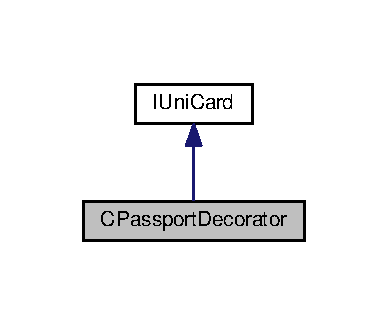
\includegraphics[width=186pt]{classCPassportDecorator__inherit__graph}
\end{center}
\end{figure}


Collaboration diagram for C\+Passport\+Decorator\+:\nopagebreak
\begin{figure}[H]
\begin{center}
\leavevmode
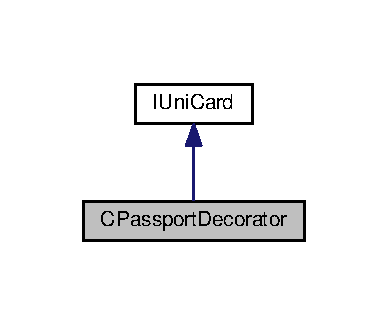
\includegraphics[width=186pt]{classCPassportDecorator__coll__graph}
\end{center}
\end{figure}
\subsection*{Public Member Functions}
\begin{DoxyCompactItemize}
\item 
\mbox{\Hypertarget{classCPassportDecorator_aa43bccb88ac663e1a36d85c567ab5076}\label{classCPassportDecorator_aa43bccb88ac663e1a36d85c567ab5076}} 
{\bfseries C\+Passport\+Decorator} (\hyperlink{classCUniCard}{C\+Uni\+Card} $\ast$\+\_\+unicard, string \+\_\+born\+Date, string \+\_\+born\+Place, string \+\_\+passport\+Available\+To\+Date)
\item 
virtual void \hyperlink{classCPassportDecorator_aec16f6c3f9feaa6da4d8cef5ea27c7b8}{info} ()
\begin{DoxyCompactList}\small\item\em Паспортные данные гражданина(ФИО, Дата и место рождения, не истек ли срок паспорта)\+: \end{DoxyCompactList}\item 
string \hyperlink{classCPassportDecorator_a116ab0fa075e02edb74339e2e1cd3389}{get\+Born\+Date} () const
\begin{DoxyCompactList}\small\item\em Дата рождения \end{DoxyCompactList}\item 
string \hyperlink{classCPassportDecorator_a941e597cc2514d8397030eab58682aa6}{get\+Born\+Place} () const
\begin{DoxyCompactList}\small\item\em Место рождения \end{DoxyCompactList}\item 
string \hyperlink{classCPassportDecorator_a96c55b65b042d4294d6cba471a936574}{get\+Passport\+Available\+To\+Date} () const
\begin{DoxyCompactList}\small\item\em Проверка истечения срока пасспорта \end{DoxyCompactList}\end{DoxyCompactItemize}
\subsection*{Public Attributes}
\begin{DoxyCompactItemize}
\item 
bool \hyperlink{classCPassportDecorator_a972d9fe88105ba06ec5bab01e230b1a8}{check\+In\+Base}
\begin{DoxyCompactList}\small\item\em Проверить на фальшивость \end{DoxyCompactList}\item 
bool \hyperlink{classCPassportDecorator_a2497ce4827a91e25a28756a56a8ba245}{check\+For\+Visa}
\begin{DoxyCompactList}\small\item\em Проверить срок визы \end{DoxyCompactList}\end{DoxyCompactItemize}


\subsection{Detailed Description}
Декоратор пасспорта 

\subsection{Member Function Documentation}
\mbox{\Hypertarget{classCPassportDecorator_a116ab0fa075e02edb74339e2e1cd3389}\label{classCPassportDecorator_a116ab0fa075e02edb74339e2e1cd3389}} 
\index{C\+Passport\+Decorator@{C\+Passport\+Decorator}!get\+Born\+Date@{get\+Born\+Date}}
\index{get\+Born\+Date@{get\+Born\+Date}!C\+Passport\+Decorator@{C\+Passport\+Decorator}}
\subsubsection{\texorpdfstring{get\+Born\+Date()}{getBornDate()}}
{\footnotesize\ttfamily string C\+Passport\+Decorator\+::get\+Born\+Date (\begin{DoxyParamCaption}{ }\end{DoxyParamCaption}) const\hspace{0.3cm}{\ttfamily [inline]}}



Дата рождения 

\begin{DoxyReturn}{Returns}
Вывод даты рождения 
\end{DoxyReturn}
\mbox{\Hypertarget{classCPassportDecorator_a941e597cc2514d8397030eab58682aa6}\label{classCPassportDecorator_a941e597cc2514d8397030eab58682aa6}} 
\index{C\+Passport\+Decorator@{C\+Passport\+Decorator}!get\+Born\+Place@{get\+Born\+Place}}
\index{get\+Born\+Place@{get\+Born\+Place}!C\+Passport\+Decorator@{C\+Passport\+Decorator}}
\subsubsection{\texorpdfstring{get\+Born\+Place()}{getBornPlace()}}
{\footnotesize\ttfamily string C\+Passport\+Decorator\+::get\+Born\+Place (\begin{DoxyParamCaption}{ }\end{DoxyParamCaption}) const\hspace{0.3cm}{\ttfamily [inline]}}



Место рождения 

\begin{DoxyReturn}{Returns}
Вывод места рождения 
\end{DoxyReturn}
\mbox{\Hypertarget{classCPassportDecorator_a96c55b65b042d4294d6cba471a936574}\label{classCPassportDecorator_a96c55b65b042d4294d6cba471a936574}} 
\index{C\+Passport\+Decorator@{C\+Passport\+Decorator}!get\+Passport\+Available\+To\+Date@{get\+Passport\+Available\+To\+Date}}
\index{get\+Passport\+Available\+To\+Date@{get\+Passport\+Available\+To\+Date}!C\+Passport\+Decorator@{C\+Passport\+Decorator}}
\subsubsection{\texorpdfstring{get\+Passport\+Available\+To\+Date()}{getPassportAvailableToDate()}}
{\footnotesize\ttfamily string C\+Passport\+Decorator\+::get\+Passport\+Available\+To\+Date (\begin{DoxyParamCaption}{ }\end{DoxyParamCaption}) const\hspace{0.3cm}{\ttfamily [inline]}}



Проверка истечения срока пасспорта 

\begin{DoxyReturn}{Returns}
Результаты проверки 
\end{DoxyReturn}
\mbox{\Hypertarget{classCPassportDecorator_aec16f6c3f9feaa6da4d8cef5ea27c7b8}\label{classCPassportDecorator_aec16f6c3f9feaa6da4d8cef5ea27c7b8}} 
\index{C\+Passport\+Decorator@{C\+Passport\+Decorator}!info@{info}}
\index{info@{info}!C\+Passport\+Decorator@{C\+Passport\+Decorator}}
\subsubsection{\texorpdfstring{info()}{info()}}
{\footnotesize\ttfamily virtual void C\+Passport\+Decorator\+::info (\begin{DoxyParamCaption}{ }\end{DoxyParamCaption})\hspace{0.3cm}{\ttfamily [inline]}, {\ttfamily [virtual]}}



Паспортные данные гражданина(ФИО, Дата и место рождения, не истек ли срок паспорта)\+: 

\begin{DoxyReturn}{Returns}
Вывод информации о переводе 
\end{DoxyReturn}


Implements \hyperlink{classIUniCard}{I\+Uni\+Card}.



\subsection{Member Data Documentation}
\mbox{\Hypertarget{classCPassportDecorator_a2497ce4827a91e25a28756a56a8ba245}\label{classCPassportDecorator_a2497ce4827a91e25a28756a56a8ba245}} 
\index{C\+Passport\+Decorator@{C\+Passport\+Decorator}!check\+For\+Visa@{check\+For\+Visa}}
\index{check\+For\+Visa@{check\+For\+Visa}!C\+Passport\+Decorator@{C\+Passport\+Decorator}}
\subsubsection{\texorpdfstring{check\+For\+Visa}{checkForVisa}}
{\footnotesize\ttfamily bool C\+Passport\+Decorator\+::check\+For\+Visa}

{\bfseries Initial value\+:}
\begin{DoxyCode}
\{
            
    \}
\end{DoxyCode}


Проверить срок визы 

\begin{DoxyReturn}{Returns}
Вывод информации 
\end{DoxyReturn}
\mbox{\Hypertarget{classCPassportDecorator_a972d9fe88105ba06ec5bab01e230b1a8}\label{classCPassportDecorator_a972d9fe88105ba06ec5bab01e230b1a8}} 
\index{C\+Passport\+Decorator@{C\+Passport\+Decorator}!check\+In\+Base@{check\+In\+Base}}
\index{check\+In\+Base@{check\+In\+Base}!C\+Passport\+Decorator@{C\+Passport\+Decorator}}
\subsubsection{\texorpdfstring{check\+In\+Base}{checkInBase}}
{\footnotesize\ttfamily bool C\+Passport\+Decorator\+::check\+In\+Base}

{\bfseries Initial value\+:}
\begin{DoxyCode}
\{
          
    \}
\end{DoxyCode}


Проверить на фальшивость 

\begin{DoxyReturn}{Returns}
Вывод информации 
\end{DoxyReturn}


The documentation for this class was generated from the following file\+:\begin{DoxyCompactItemize}
\item 
C\+Passport\+Decorator.\+h\end{DoxyCompactItemize}

\hypertarget{classCPassportReader}{}\section{C\+Passport\+Reader Class Reference}
\label{classCPassportReader}\index{C\+Passport\+Reader@{C\+Passport\+Reader}}


Интерфейс Device, считающего паспорт  




{\ttfamily \#include $<$C\+Passport\+Reader.\+h$>$}



Inheritance diagram for C\+Passport\+Reader\+:\nopagebreak
\begin{figure}[H]
\begin{center}
\leavevmode
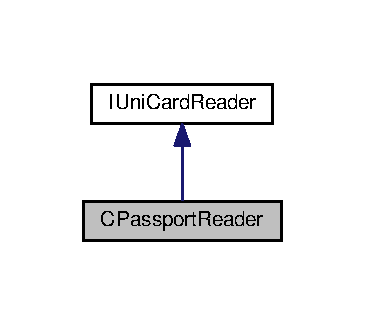
\includegraphics[width=175pt]{classCPassportReader__inherit__graph}
\end{center}
\end{figure}


Collaboration diagram for C\+Passport\+Reader\+:\nopagebreak
\begin{figure}[H]
\begin{center}
\leavevmode
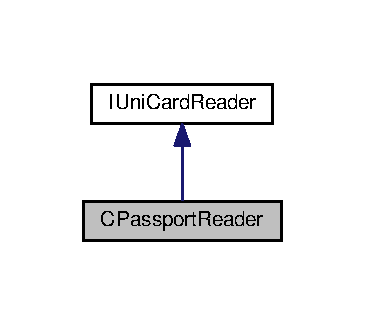
\includegraphics[width=175pt]{classCPassportReader__coll__graph}
\end{center}
\end{figure}
\subsection*{Public Member Functions}
\begin{DoxyCompactItemize}
\item 
\mbox{\Hypertarget{classCPassportReader_acda8f2f99e534bbe80f96cab38e80ab9}\label{classCPassportReader_acda8f2f99e534bbe80f96cab38e80ab9}} 
{\bfseries C\+Passport\+Reader} (\hyperlink{classCPassportDecorator}{C\+Passport\+Decorator} $\ast$\+\_\+unicard)
\item 
\mbox{\Hypertarget{classCPassportReader_a62ed2b4972b4cebd1ebaeb594d04fa9c}\label{classCPassportReader_a62ed2b4972b4cebd1ebaeb594d04fa9c}} 
virtual void \hyperlink{classCPassportReader_a62ed2b4972b4cebd1ebaeb594d04fa9c}{reader} ()
\begin{DoxyCompactList}\small\item\em Общая информация о карте \end{DoxyCompactList}\end{DoxyCompactItemize}


\subsection{Detailed Description}
Интерфейс Device, считающего паспорт 

The documentation for this class was generated from the following file\+:\begin{DoxyCompactItemize}
\item 
C\+Passport\+Reader.\+h\end{DoxyCompactItemize}

\hypertarget{classCPolisDecorator}{}\section{C\+Polis\+Decorator Class Reference}
\label{classCPolisDecorator}\index{C\+Polis\+Decorator@{C\+Polis\+Decorator}}


Декоратор страхового полиса  




{\ttfamily \#include $<$C\+Polis\+Decorator.\+h$>$}



Inheritance diagram for C\+Polis\+Decorator\+:\nopagebreak
\begin{figure}[H]
\begin{center}
\leavevmode
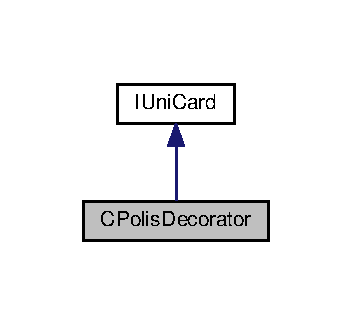
\includegraphics[width=169pt]{classCPolisDecorator__inherit__graph}
\end{center}
\end{figure}


Collaboration diagram for C\+Polis\+Decorator\+:\nopagebreak
\begin{figure}[H]
\begin{center}
\leavevmode
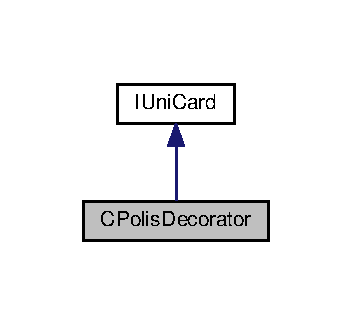
\includegraphics[width=169pt]{classCPolisDecorator__coll__graph}
\end{center}
\end{figure}
\subsection*{Public Member Functions}
\begin{DoxyCompactItemize}
\item 
\mbox{\Hypertarget{classCPolisDecorator_a7ae702036d0fc6d91178f25a4f00d64c}\label{classCPolisDecorator_a7ae702036d0fc6d91178f25a4f00d64c}} 
{\bfseries C\+Polis\+Decorator} (shared\+\_\+ptr$<$ \hyperlink{classCUniCard}{C\+Uni\+Card} $>$ \+\_\+unicard, string \+\_\+born\+Date, string \+\_\+last\+Visit)
\item 
virtual void \hyperlink{classCPolisDecorator_a3e5c7651e0db69bfcc4a9b67e961b9a8}{info} ()
\begin{DoxyCompactList}\small\item\em Основная информация по полису\+: \end{DoxyCompactList}\item 
string \hyperlink{classCPolisDecorator_a9e380f2e7020eb4444a0bb3747380918}{get\+Age} () const
\begin{DoxyCompactList}\small\item\em Дата рождения \end{DoxyCompactList}\item 
string \hyperlink{classCPolisDecorator_afc603d0d42eb72689b103bd47ec225ce}{get\+Last\+Visit} () const
\begin{DoxyCompactList}\small\item\em Дата последнего визита к врачу \end{DoxyCompactList}\item 
vector$<$ string $>$ \hyperlink{classCPolisDecorator_ac43dd7017dc2a1dd70d2cf0431cc3e7f}{get\+Ilnesses} () const
\begin{DoxyCompactList}\small\item\em Список болезней \end{DoxyCompactList}\item 
\mbox{\Hypertarget{classCPolisDecorator_a473a2c0b0bba20c7fc8575a7aae5a5ae}\label{classCPolisDecorator_a473a2c0b0bba20c7fc8575a7aae5a5ae}} 
void {\bfseries print\+Ilnesses} () const
\end{DoxyCompactItemize}
\subsection*{Public Attributes}
\begin{DoxyCompactItemize}
\item 
bool \hyperlink{classCPolisDecorator_adc7849b17854791c53ae1b18a7b445c6}{check\+In\+Base}
\begin{DoxyCompactList}\small\item\em Проверить прикреплен ли человек \end{DoxyCompactList}\item 
bool \hyperlink{classCPolisDecorator_a06749afa01826039c719984b3728860a}{check\+For\+Benefits}
\begin{DoxyCompactList}\small\item\em проверить наличие льготных прав в базе. \end{DoxyCompactList}\end{DoxyCompactItemize}


\subsection{Detailed Description}
Декоратор страхового полиса 

\subsection{Member Function Documentation}
\mbox{\Hypertarget{classCPolisDecorator_a9e380f2e7020eb4444a0bb3747380918}\label{classCPolisDecorator_a9e380f2e7020eb4444a0bb3747380918}} 
\index{C\+Polis\+Decorator@{C\+Polis\+Decorator}!get\+Age@{get\+Age}}
\index{get\+Age@{get\+Age}!C\+Polis\+Decorator@{C\+Polis\+Decorator}}
\subsubsection{\texorpdfstring{get\+Age()}{getAge()}}
{\footnotesize\ttfamily string C\+Polis\+Decorator\+::get\+Age (\begin{DoxyParamCaption}{ }\end{DoxyParamCaption}) const\hspace{0.3cm}{\ttfamily [inline]}}



Дата рождения 

\begin{DoxyReturn}{Returns}
Вывод даты рождения 
\end{DoxyReturn}
\mbox{\Hypertarget{classCPolisDecorator_ac43dd7017dc2a1dd70d2cf0431cc3e7f}\label{classCPolisDecorator_ac43dd7017dc2a1dd70d2cf0431cc3e7f}} 
\index{C\+Polis\+Decorator@{C\+Polis\+Decorator}!get\+Ilnesses@{get\+Ilnesses}}
\index{get\+Ilnesses@{get\+Ilnesses}!C\+Polis\+Decorator@{C\+Polis\+Decorator}}
\subsubsection{\texorpdfstring{get\+Ilnesses()}{getIlnesses()}}
{\footnotesize\ttfamily vector$<$string$>$ C\+Polis\+Decorator\+::get\+Ilnesses (\begin{DoxyParamCaption}{ }\end{DoxyParamCaption}) const\hspace{0.3cm}{\ttfamily [inline]}}



Список болезней 

\begin{DoxyReturn}{Returns}
Вывод списка болезней 
\end{DoxyReturn}
\mbox{\Hypertarget{classCPolisDecorator_afc603d0d42eb72689b103bd47ec225ce}\label{classCPolisDecorator_afc603d0d42eb72689b103bd47ec225ce}} 
\index{C\+Polis\+Decorator@{C\+Polis\+Decorator}!get\+Last\+Visit@{get\+Last\+Visit}}
\index{get\+Last\+Visit@{get\+Last\+Visit}!C\+Polis\+Decorator@{C\+Polis\+Decorator}}
\subsubsection{\texorpdfstring{get\+Last\+Visit()}{getLastVisit()}}
{\footnotesize\ttfamily string C\+Polis\+Decorator\+::get\+Last\+Visit (\begin{DoxyParamCaption}{ }\end{DoxyParamCaption}) const\hspace{0.3cm}{\ttfamily [inline]}}



Дата последнего визита к врачу 

\begin{DoxyReturn}{Returns}
Вывод информации о последнем визите 
\end{DoxyReturn}
\mbox{\Hypertarget{classCPolisDecorator_a3e5c7651e0db69bfcc4a9b67e961b9a8}\label{classCPolisDecorator_a3e5c7651e0db69bfcc4a9b67e961b9a8}} 
\index{C\+Polis\+Decorator@{C\+Polis\+Decorator}!info@{info}}
\index{info@{info}!C\+Polis\+Decorator@{C\+Polis\+Decorator}}
\subsubsection{\texorpdfstring{info()}{info()}}
{\footnotesize\ttfamily virtual void C\+Polis\+Decorator\+::info (\begin{DoxyParamCaption}{ }\end{DoxyParamCaption})\hspace{0.3cm}{\ttfamily [inline]}, {\ttfamily [virtual]}}



Основная информация по полису\+: 

Возраст, дата последнего визита, список болезней \begin{DoxyReturn}{Returns}
Вывод информации по полису 
\end{DoxyReturn}


Implements \hyperlink{classIUniCard}{I\+Uni\+Card}.



\subsection{Member Data Documentation}
\mbox{\Hypertarget{classCPolisDecorator_a06749afa01826039c719984b3728860a}\label{classCPolisDecorator_a06749afa01826039c719984b3728860a}} 
\index{C\+Polis\+Decorator@{C\+Polis\+Decorator}!check\+For\+Benefits@{check\+For\+Benefits}}
\index{check\+For\+Benefits@{check\+For\+Benefits}!C\+Polis\+Decorator@{C\+Polis\+Decorator}}
\subsubsection{\texorpdfstring{check\+For\+Benefits}{checkForBenefits}}
{\footnotesize\ttfamily bool C\+Polis\+Decorator\+::check\+For\+Benefits}

{\bfseries Initial value\+:}
\begin{DoxyCode}
\{
            
    \}
\end{DoxyCode}


проверить наличие льготных прав в базе. 

\begin{DoxyReturn}{Returns}
Вывод информации о льготах 
\end{DoxyReturn}
\mbox{\Hypertarget{classCPolisDecorator_adc7849b17854791c53ae1b18a7b445c6}\label{classCPolisDecorator_adc7849b17854791c53ae1b18a7b445c6}} 
\index{C\+Polis\+Decorator@{C\+Polis\+Decorator}!check\+In\+Base@{check\+In\+Base}}
\index{check\+In\+Base@{check\+In\+Base}!C\+Polis\+Decorator@{C\+Polis\+Decorator}}
\subsubsection{\texorpdfstring{check\+In\+Base}{checkInBase}}
{\footnotesize\ttfamily bool C\+Polis\+Decorator\+::check\+In\+Base}

{\bfseries Initial value\+:}
\begin{DoxyCode}
\{
            
    \}
\end{DoxyCode}


Проверить прикреплен ли человек 

\begin{DoxyReturn}{Returns}
Вывод информации 
\end{DoxyReturn}


The documentation for this class was generated from the following file\+:\begin{DoxyCompactItemize}
\item 
C\+Polis\+Decorator.\+h\end{DoxyCompactItemize}

\hypertarget{classCPolisReader}{}\section{C\+Polis\+Reader Class Reference}
\label{classCPolisReader}\index{C\+Polis\+Reader@{C\+Polis\+Reader}}


Интерфейс Device, считающего страховой полис  




{\ttfamily \#include $<$C\+Polis\+Reader.\+h$>$}



Inheritance diagram for C\+Polis\+Reader\+:\nopagebreak
\begin{figure}[H]
\begin{center}
\leavevmode
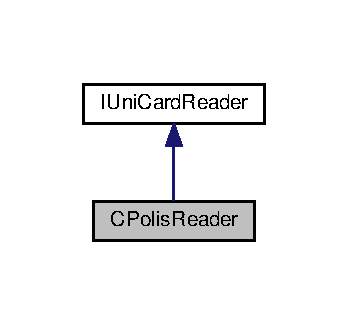
\includegraphics[width=167pt]{classCPolisReader__inherit__graph}
\end{center}
\end{figure}


Collaboration diagram for C\+Polis\+Reader\+:\nopagebreak
\begin{figure}[H]
\begin{center}
\leavevmode
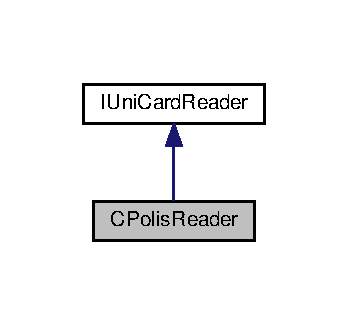
\includegraphics[width=167pt]{classCPolisReader__coll__graph}
\end{center}
\end{figure}
\subsection*{Public Member Functions}
\begin{DoxyCompactItemize}
\item 
\mbox{\Hypertarget{classCPolisReader_a8adfeca19ec5f6919209ca579f1e5cf3}\label{classCPolisReader_a8adfeca19ec5f6919209ca579f1e5cf3}} 
{\bfseries C\+Polis\+Reader} (\hyperlink{classCPolisDecorator}{C\+Polis\+Decorator} $\ast$\+\_\+unicard)
\item 
\mbox{\Hypertarget{classCPolisReader_a8c56b8c31bb1587d7cd4cc0225eaa41e}\label{classCPolisReader_a8c56b8c31bb1587d7cd4cc0225eaa41e}} 
virtual void \hyperlink{classCPolisReader_a8c56b8c31bb1587d7cd4cc0225eaa41e}{reader} ()
\begin{DoxyCompactList}\small\item\em Вывод информации про данную карту \end{DoxyCompactList}\end{DoxyCompactItemize}


\subsection{Detailed Description}
Интерфейс Device, считающего страховой полис 

The documentation for this class was generated from the following file\+:\begin{DoxyCompactItemize}
\item 
C\+Polis\+Reader.\+h\end{DoxyCompactItemize}

\hypertarget{classCSberbankDecorator}{}\section{C\+Sberbank\+Decorator Class Reference}
\label{classCSberbankDecorator}\index{C\+Sberbank\+Decorator@{C\+Sberbank\+Decorator}}


Декоратор сбербанковской карты  




{\ttfamily \#include $<$C\+Sberbank\+Decorator.\+h$>$}



Inheritance diagram for C\+Sberbank\+Decorator\+:\nopagebreak
\begin{figure}[H]
\begin{center}
\leavevmode
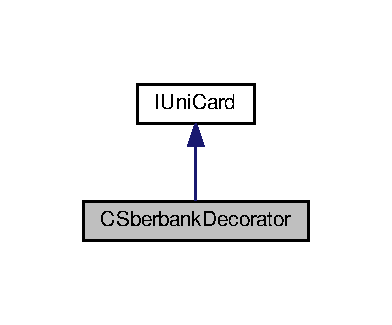
\includegraphics[width=188pt]{classCSberbankDecorator__inherit__graph}
\end{center}
\end{figure}


Collaboration diagram for C\+Sberbank\+Decorator\+:\nopagebreak
\begin{figure}[H]
\begin{center}
\leavevmode
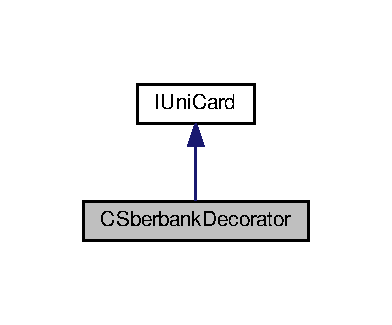
\includegraphics[width=188pt]{classCSberbankDecorator__coll__graph}
\end{center}
\end{figure}
\subsection*{Public Member Functions}
\begin{DoxyCompactItemize}
\item 
\mbox{\Hypertarget{classCSberbankDecorator_a0cab61c44399947bbe5355a2fb70428f}\label{classCSberbankDecorator_a0cab61c44399947bbe5355a2fb70428f}} 
{\bfseries C\+Sberbank\+Decorator} (\hyperlink{classCUniCard}{C\+Uni\+Card} $\ast$\+\_\+unicard, int \+\_\+money, bool \+\_\+available)
\item 
\mbox{\Hypertarget{classCSberbankDecorator_a253d67f88793c4e6ce5698e616cdeb07}\label{classCSberbankDecorator_a253d67f88793c4e6ce5698e616cdeb07}} 
int {\bfseries get\+Money} () const
\item 
\mbox{\Hypertarget{classCSberbankDecorator_ab69d38128eb4ba05d2d5b21769b80204}\label{classCSberbankDecorator_ab69d38128eb4ba05d2d5b21769b80204}} 
bool {\bfseries check\+Available} () const
\item 
\mbox{\Hypertarget{classCSberbankDecorator_a51576c6acd9000635528d0d414fcd053}\label{classCSberbankDecorator_a51576c6acd9000635528d0d414fcd053}} 
void {\bfseries set\+Money} (int value)
\item 
virtual void \hyperlink{classCSberbankDecorator_a2c19e1fe10123e813de29572512d69b8}{info} ()
\begin{DoxyCompactList}\small\item\em Платежная информация по карте \end{DoxyCompactList}\item 
void \hyperlink{classCSberbankDecorator_a6c8175379ec2e07e6b4fe6fe2da58425}{send\+Money} (int value)
\begin{DoxyCompactList}\small\item\em Перевод денежных средств другому клиенту \end{DoxyCompactList}\item 
void \hyperlink{classCSberbankDecorator_a4182d5c8d8d0214ad53c26ebe26cce09}{get\+Money\+From\+Other} (int value)
\begin{DoxyCompactList}\small\item\em Получение денежных средств от другого клиента \end{DoxyCompactList}\item 
void \hyperlink{classCSberbankDecorator_a60aedba1baefb930f51176b38d3682c5}{check\+Hipotecs} ()
\begin{DoxyCompactList}\small\item\em Проверка задолженностей и ипотек \end{DoxyCompactList}\item 
void \hyperlink{classCSberbankDecorator_a0bee1976bcb32c4e927166aa3ab857d0}{check\+Deposit} ()
\begin{DoxyCompactList}\small\item\em Проверка депозитных счетов \end{DoxyCompactList}\end{DoxyCompactItemize}


\subsection{Detailed Description}
Декоратор сбербанковской карты 

\subsection{Member Function Documentation}
\mbox{\Hypertarget{classCSberbankDecorator_a0bee1976bcb32c4e927166aa3ab857d0}\label{classCSberbankDecorator_a0bee1976bcb32c4e927166aa3ab857d0}} 
\index{C\+Sberbank\+Decorator@{C\+Sberbank\+Decorator}!check\+Deposit@{check\+Deposit}}
\index{check\+Deposit@{check\+Deposit}!C\+Sberbank\+Decorator@{C\+Sberbank\+Decorator}}
\subsubsection{\texorpdfstring{check\+Deposit()}{checkDeposit()}}
{\footnotesize\ttfamily void C\+Sberbank\+Decorator\+::check\+Deposit (\begin{DoxyParamCaption}{ }\end{DoxyParamCaption})\hspace{0.3cm}{\ttfamily [inline]}}



Проверка депозитных счетов 

\begin{DoxyReturn}{Returns}
Вывод информации о вкладах 
\end{DoxyReturn}
\mbox{\Hypertarget{classCSberbankDecorator_a60aedba1baefb930f51176b38d3682c5}\label{classCSberbankDecorator_a60aedba1baefb930f51176b38d3682c5}} 
\index{C\+Sberbank\+Decorator@{C\+Sberbank\+Decorator}!check\+Hipotecs@{check\+Hipotecs}}
\index{check\+Hipotecs@{check\+Hipotecs}!C\+Sberbank\+Decorator@{C\+Sberbank\+Decorator}}
\subsubsection{\texorpdfstring{check\+Hipotecs()}{checkHipotecs()}}
{\footnotesize\ttfamily void C\+Sberbank\+Decorator\+::check\+Hipotecs (\begin{DoxyParamCaption}{ }\end{DoxyParamCaption})\hspace{0.3cm}{\ttfamily [inline]}}



Проверка задолженностей и ипотек 

\begin{DoxyReturn}{Returns}
Вывод информации о долгах и ипотеках 
\end{DoxyReturn}
\mbox{\Hypertarget{classCSberbankDecorator_a4182d5c8d8d0214ad53c26ebe26cce09}\label{classCSberbankDecorator_a4182d5c8d8d0214ad53c26ebe26cce09}} 
\index{C\+Sberbank\+Decorator@{C\+Sberbank\+Decorator}!get\+Money\+From\+Other@{get\+Money\+From\+Other}}
\index{get\+Money\+From\+Other@{get\+Money\+From\+Other}!C\+Sberbank\+Decorator@{C\+Sberbank\+Decorator}}
\subsubsection{\texorpdfstring{get\+Money\+From\+Other()}{getMoneyFromOther()}}
{\footnotesize\ttfamily void C\+Sberbank\+Decorator\+::get\+Money\+From\+Other (\begin{DoxyParamCaption}\item[{int}]{value }\end{DoxyParamCaption})\hspace{0.3cm}{\ttfamily [inline]}}



Получение денежных средств от другого клиента 

\begin{DoxyReturn}{Returns}
Вывод информации о получении 
\end{DoxyReturn}
\mbox{\Hypertarget{classCSberbankDecorator_a2c19e1fe10123e813de29572512d69b8}\label{classCSberbankDecorator_a2c19e1fe10123e813de29572512d69b8}} 
\index{C\+Sberbank\+Decorator@{C\+Sberbank\+Decorator}!info@{info}}
\index{info@{info}!C\+Sberbank\+Decorator@{C\+Sberbank\+Decorator}}
\subsubsection{\texorpdfstring{info()}{info()}}
{\footnotesize\ttfamily virtual void C\+Sberbank\+Decorator\+::info (\begin{DoxyParamCaption}{ }\end{DoxyParamCaption})\hspace{0.3cm}{\ttfamily [inline]}, {\ttfamily [virtual]}}



Платежная информация по карте 

\begin{DoxyReturn}{Returns}
Вывод информации о владельце карты 
\end{DoxyReturn}


Implements \hyperlink{classIUniCard}{I\+Uni\+Card}.

\mbox{\Hypertarget{classCSberbankDecorator_a6c8175379ec2e07e6b4fe6fe2da58425}\label{classCSberbankDecorator_a6c8175379ec2e07e6b4fe6fe2da58425}} 
\index{C\+Sberbank\+Decorator@{C\+Sberbank\+Decorator}!send\+Money@{send\+Money}}
\index{send\+Money@{send\+Money}!C\+Sberbank\+Decorator@{C\+Sberbank\+Decorator}}
\subsubsection{\texorpdfstring{send\+Money()}{sendMoney()}}
{\footnotesize\ttfamily void C\+Sberbank\+Decorator\+::send\+Money (\begin{DoxyParamCaption}\item[{int}]{value }\end{DoxyParamCaption})\hspace{0.3cm}{\ttfamily [inline]}}



Перевод денежных средств другому клиенту 

\begin{DoxyReturn}{Returns}
Вывод информации о переводе 
\end{DoxyReturn}


The documentation for this class was generated from the following file\+:\begin{DoxyCompactItemize}
\item 
C\+Sberbank\+Decorator.\+h\end{DoxyCompactItemize}

\hypertarget{classCSberbankReader}{}\section{C\+Sberbank\+Reader Class Reference}
\label{classCSberbankReader}\index{C\+Sberbank\+Reader@{C\+Sberbank\+Reader}}


Интерфейс Device, считающего карточку Сбербанка  




{\ttfamily \#include $<$C\+Sberbank\+Reader.\+h$>$}



Inheritance diagram for C\+Sberbank\+Reader\+:\nopagebreak
\begin{figure}[H]
\begin{center}
\leavevmode
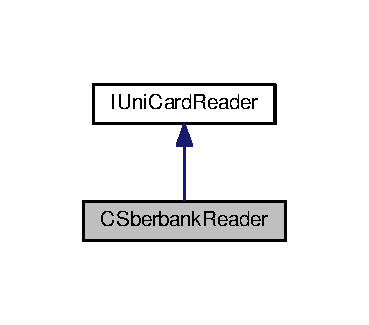
\includegraphics[width=177pt]{classCSberbankReader__inherit__graph}
\end{center}
\end{figure}


Collaboration diagram for C\+Sberbank\+Reader\+:\nopagebreak
\begin{figure}[H]
\begin{center}
\leavevmode
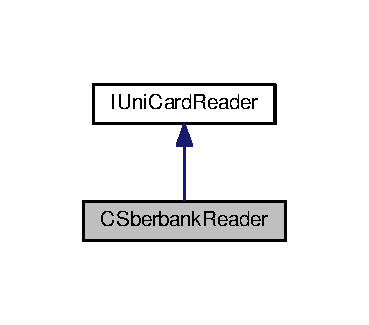
\includegraphics[width=177pt]{classCSberbankReader__coll__graph}
\end{center}
\end{figure}
\subsection*{Public Member Functions}
\begin{DoxyCompactItemize}
\item 
\mbox{\Hypertarget{classCSberbankReader_abf9c9be6b446d32f681ff5f80576c5f0}\label{classCSberbankReader_abf9c9be6b446d32f681ff5f80576c5f0}} 
{\bfseries C\+Sberbank\+Reader} (\hyperlink{classCSberbankDecorator}{C\+Sberbank\+Decorator} $\ast$\+\_\+unicard)
\item 
\mbox{\Hypertarget{classCSberbankReader_a4dd1f87a1f3272b9028605f00518194b}\label{classCSberbankReader_a4dd1f87a1f3272b9028605f00518194b}} 
virtual void \hyperlink{classCSberbankReader_a4dd1f87a1f3272b9028605f00518194b}{reader} ()
\begin{DoxyCompactList}\small\item\em Общая информация о карте \end{DoxyCompactList}\item 
void \hyperlink{classCSberbankReader_a8956f7c08e0bbffc81f432d4fe3408f3}{send\+Money} (int \+\_\+value)
\begin{DoxyCompactList}\small\item\em Перевод денежных средств другому клиенту \end{DoxyCompactList}\item 
void \hyperlink{classCSberbankReader_ad68d4071db0050cc18b0a79fcfa1c2f9}{get\+Money} (int \+\_\+value)
\begin{DoxyCompactList}\small\item\em Перевод денежных средств от другого клиенту данному \end{DoxyCompactList}\end{DoxyCompactItemize}


\subsection{Detailed Description}
Интерфейс Device, считающего карточку Сбербанка 

\subsection{Member Function Documentation}
\mbox{\Hypertarget{classCSberbankReader_ad68d4071db0050cc18b0a79fcfa1c2f9}\label{classCSberbankReader_ad68d4071db0050cc18b0a79fcfa1c2f9}} 
\index{C\+Sberbank\+Reader@{C\+Sberbank\+Reader}!get\+Money@{get\+Money}}
\index{get\+Money@{get\+Money}!C\+Sberbank\+Reader@{C\+Sberbank\+Reader}}
\subsubsection{\texorpdfstring{get\+Money()}{getMoney()}}
{\footnotesize\ttfamily void C\+Sberbank\+Reader\+::get\+Money (\begin{DoxyParamCaption}\item[{int}]{\+\_\+value }\end{DoxyParamCaption})\hspace{0.3cm}{\ttfamily [inline]}}



Перевод денежных средств от другого клиенту данному 

\begin{DoxyReturn}{Returns}
Вывод информации о получении 
\end{DoxyReturn}
\mbox{\Hypertarget{classCSberbankReader_a8956f7c08e0bbffc81f432d4fe3408f3}\label{classCSberbankReader_a8956f7c08e0bbffc81f432d4fe3408f3}} 
\index{C\+Sberbank\+Reader@{C\+Sberbank\+Reader}!send\+Money@{send\+Money}}
\index{send\+Money@{send\+Money}!C\+Sberbank\+Reader@{C\+Sberbank\+Reader}}
\subsubsection{\texorpdfstring{send\+Money()}{sendMoney()}}
{\footnotesize\ttfamily void C\+Sberbank\+Reader\+::send\+Money (\begin{DoxyParamCaption}\item[{int}]{\+\_\+value }\end{DoxyParamCaption})\hspace{0.3cm}{\ttfamily [inline]}}



Перевод денежных средств другому клиенту 

\begin{DoxyReturn}{Returns}
Вывод информации о переводе 
\end{DoxyReturn}


The documentation for this class was generated from the following file\+:\begin{DoxyCompactItemize}
\item 
C\+Sberbank\+Reader.\+h\end{DoxyCompactItemize}

\hypertarget{classCUniCard}{}\section{C\+Uni\+Card Class Reference}
\label{classCUniCard}\index{C\+Uni\+Card@{C\+Uni\+Card}}


Интерфейс Uni\+Card.  




{\ttfamily \#include $<$C\+Uni\+Card.\+h$>$}



Inheritance diagram for C\+Uni\+Card\+:\nopagebreak
\begin{figure}[H]
\begin{center}
\leavevmode
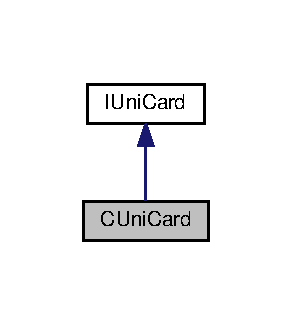
\includegraphics[width=140pt]{classCUniCard__inherit__graph}
\end{center}
\end{figure}


Collaboration diagram for C\+Uni\+Card\+:\nopagebreak
\begin{figure}[H]
\begin{center}
\leavevmode
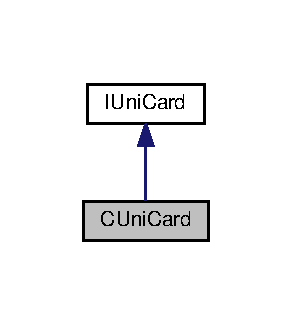
\includegraphics[width=140pt]{classCUniCard__coll__graph}
\end{center}
\end{figure}
\subsection*{Public Member Functions}
\begin{DoxyCompactItemize}
\item 
\mbox{\Hypertarget{classCUniCard_a572470efc8f60cb742347ac1899e5e0f}\label{classCUniCard_a572470efc8f60cb742347ac1899e5e0f}} 
{\bfseries C\+Uni\+Card} (std\+::string \+\_\+client\+ID, std\+::string \+\_\+client\+Name)
\item 
\mbox{\Hypertarget{classCUniCard_a27e7269800748f3dadeaecef60d0d6c3}\label{classCUniCard_a27e7269800748f3dadeaecef60d0d6c3}} 
std\+::string {\bfseries get\+Client\+ID} () const
\item 
\mbox{\Hypertarget{classCUniCard_aecbc839e2f73e8fac5f1c0216d4ac7bf}\label{classCUniCard_aecbc839e2f73e8fac5f1c0216d4ac7bf}} 
std\+::string {\bfseries get\+Client\+Name} () const
\item 
virtual void \hyperlink{classCUniCard_ae9fe7cef81ddff409a20b1aeddb45fa9}{info} ()
\begin{DoxyCompactList}\small\item\em Информация о владельце карты \end{DoxyCompactList}\end{DoxyCompactItemize}


\subsection{Detailed Description}
Интерфейс Uni\+Card. 

\subsection{Member Function Documentation}
\mbox{\Hypertarget{classCUniCard_ae9fe7cef81ddff409a20b1aeddb45fa9}\label{classCUniCard_ae9fe7cef81ddff409a20b1aeddb45fa9}} 
\index{C\+Uni\+Card@{C\+Uni\+Card}!info@{info}}
\index{info@{info}!C\+Uni\+Card@{C\+Uni\+Card}}
\subsubsection{\texorpdfstring{info()}{info()}}
{\footnotesize\ttfamily virtual void C\+Uni\+Card\+::info (\begin{DoxyParamCaption}{ }\end{DoxyParamCaption})\hspace{0.3cm}{\ttfamily [inline]}, {\ttfamily [virtual]}}



Информация о владельце карты 

\begin{DoxyReturn}{Returns}
Вывод информации о владельце 
\end{DoxyReturn}


Implements \hyperlink{classIUniCard}{I\+Uni\+Card}.



The documentation for this class was generated from the following file\+:\begin{DoxyCompactItemize}
\item 
C\+Uni\+Card.\+h\end{DoxyCompactItemize}

\hypertarget{classIUniCard}{}\section{I\+Uni\+Card Class Reference}
\label{classIUniCard}\index{I\+Uni\+Card@{I\+Uni\+Card}}


интерфейс Uni\+Card.  




{\ttfamily \#include $<$I\+Uni\+Card.\+h$>$}



Inheritance diagram for I\+Uni\+Card\+:\nopagebreak
\begin{figure}[H]
\begin{center}
\leavevmode
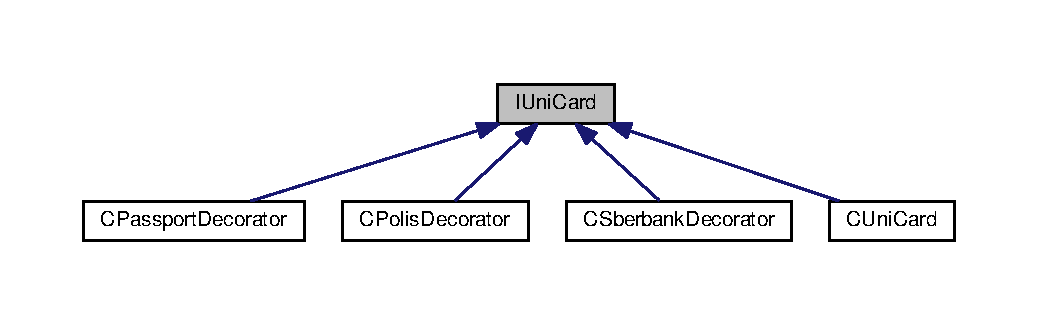
\includegraphics[width=350pt]{classIUniCard__inherit__graph}
\end{center}
\end{figure}
\subsection*{Public Member Functions}
\begin{DoxyCompactItemize}
\item 
\mbox{\Hypertarget{classIUniCard_ae2f691f3ca5879965692d9061f88c423}\label{classIUniCard_ae2f691f3ca5879965692d9061f88c423}} 
virtual void {\bfseries info} ()=0
\end{DoxyCompactItemize}


\subsection{Detailed Description}
интерфейс Uni\+Card. 

The documentation for this class was generated from the following file\+:\begin{DoxyCompactItemize}
\item 
I\+Uni\+Card.\+h\end{DoxyCompactItemize}

\hypertarget{classIUniCardReader}{}\section{I\+Uni\+Card\+Reader Class Reference}
\label{classIUniCardReader}\index{I\+Uni\+Card\+Reader@{I\+Uni\+Card\+Reader}}


Интерфейс Считающего устройства(device)  




{\ttfamily \#include $<$I\+Uni\+Card\+Reader.\+h$>$}



Inheritance diagram for I\+Uni\+Card\+Reader\+:\nopagebreak
\begin{figure}[H]
\begin{center}
\leavevmode
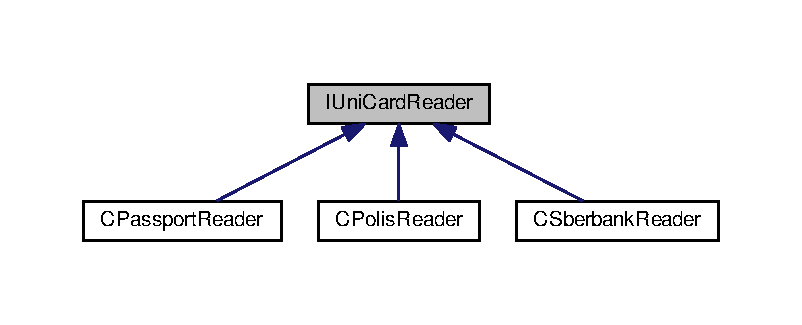
\includegraphics[width=350pt]{classIUniCardReader__inherit__graph}
\end{center}
\end{figure}
\subsection*{Public Member Functions}
\begin{DoxyCompactItemize}
\item 
\mbox{\Hypertarget{classIUniCardReader_abcfe21ca7541476fa85275c489d84f91}\label{classIUniCardReader_abcfe21ca7541476fa85275c489d84f91}} 
virtual void {\bfseries reader} ()=0
\end{DoxyCompactItemize}


\subsection{Detailed Description}
Интерфейс Считающего устройства(device) 

The documentation for this class was generated from the following file\+:\begin{DoxyCompactItemize}
\item 
I\+Uni\+Card\+Reader.\+h\end{DoxyCompactItemize}

%--- End generated contents ---

% Index
\backmatter
\newpage
\phantomsection
\clearemptydoublepage
\addcontentsline{toc}{chapter}{Index}
\printindex

\end{document}
